\documentclass[11pt]{article}
\usepackage[margin=1.0in]{geometry}
\usepackage{amsmath,amssymb,bm}
\usepackage{booktabs}
\usepackage{longtable}
\usepackage{array}
\usepackage{xcolor}
\usepackage{enumitem}
\usepackage{tikz}
\usepackage{adjustbox}
\usetikzlibrary{arrows.meta,positioning,shapes.geometric,calc,fit,backgrounds}
\usepackage{hyperref}
\hypersetup{colorlinks=true, linkcolor=blue!55!black, urlcolor=blue!55!black}

% ---- data-flow-diagram vocabulary --------------------------------------
\definecolor{procfill}{RGB}{226,238,250}
\definecolor{storefill}{RGB}{255,246,214}
\definecolor{extfill}{RGB}{232,232,232}
\definecolor{gatefill}{RGB}{226,245,226}
\tikzset{
  proc/.style  ={draw, rounded corners=6pt, fill=procfill, align=center, font=\small, inner sep=4pt, minimum height=9mm},
  store/.style ={draw, fill=storefill, align=center, font=\small\ttfamily, inner sep=3pt, minimum height=7mm,
                 path picture={\draw[line width=1.2pt] (path picture bounding box.north west) -- (path picture bounding box.south west);}},
  ext/.style   ={draw, fill=extfill, align=center, font=\small, inner sep=4pt, minimum height=9mm},
  gate/.style  ={draw, diamond, aspect=2.2, fill=gatefill, align=center, font=\small, inner sep=1pt},
  flow/.style  ={-{Stealth[length=2.2mm]}, line width=0.6pt},
  lbl/.style   ={font=\scriptsize, fill=white, inner sep=1pt, align=center}
}
% file and function names are long: let them break after an underscore
\renewcommand{\_}{\textunderscore\allowbreak}
\newcolumntype{L}[1]{>{\raggedright\arraybackslash}p{#1}}
\newcommand{\code}[1]{\texttt{#1}}
\newcommand{\file}[1]{\texttt{\small #1}}

\title{\code{reproduce\_library\_70mN}:\\[2pt] \large Rebuilding the 70\,mN DRO\,$\to$\,Tulip Costate Library\\ Software Design Document}
\author{M.~Casey}
\date{September 19, 2026}

\begin{document}
\maketitle

\begin{abstract}
\noindent\sloppy
The script \code{reproduce\_library\_70mN} is one MATLAB function that rebuilds the
70\,mN DRO\,$\to$\,tulip minimum-time costate library from its anchors,
unattended, and then checks the result, cell by cell, against the library
of record. This document says what the script does, how data moves through
it, which processes and files exist while it runs, how long it takes, what
its verdict means, and where it is weak. It is written to be read by a
person who has not seen the code. The first full run (2026-09-18/19, 24\,h
12\,min) produced a complete library that matches the hand-built record in
565 of 576 cells and is \emph{faster} in the other 11; that library is now
the record.
\end{abstract}

\tableofcontents
\newpage

% =========================================================================
\section{What this software is for}

\paragraph{The product.} A \emph{costate library} is a table of solved
minimum-time low-thrust transfers between two periodic orbits of the
Earth--Moon circular restricted three-body problem. Each entry is one
transfer: from the point at \emph{departure phase} $s_D$ on a distant
retrograde orbit (DRO) to the point at \emph{arrival phase} $s_A$ on a
7-petal tulip orbit, with a 70\,mN engine always on. An entry stores the
eight numbers that reproduce the whole trajectory,
\[
  z_8=\big[\,\bm\lambda(0)\;;\;t_f\,\big],
\]
the seven initial costates of Pontryagin's principle and the flight time.
A phase is a fraction of the orbit's period, in $[0,1)$. The library covers
a grid of $24\times24$ phase pairs: 576 transfers, each certified.

\paragraph{Why a script.} The library of record was first built by hand
over eight rounds and three days (2026-09-13 to 09-15): arcs walked, a
sheet built, gaps found, a new solution family discovered, and round again.
That process cannot be repeated by someone else, and nothing proved the
result could be recovered. The script turns it into one call whose output
is compared, automatically, with what it is meant to reproduce.

\paragraph{What it is not.} It rebuilds \emph{this} library: one engine,
one orbit pair. It starts from five solutions that are already known
(\S\ref{sec:inputs}). It is not yet a generator for a new orbit pair or a
new engine; \S\ref{sec:extend} says what that would take.

\subsection{Three ways to call it}

\begin{description}[leftmargin=0.6cm, style=nextline, itemsep=3pt]
\item[\code{reproduce\_library\_70mN}]
  \textbf{Plan.} Prints the problem, the five families, the arcs and seed
  roots found on disk, and a time estimate. Creates nothing.
\item[\code{reproduce\_library\_70mN(struct('go',true))}]
  \textbf{Build}, then compare, then print a verdict. About one day.
\item[\code{reproduce\_library\_70mN(struct('compareOnly',true))}]
  \textbf{Compare} a finished build with the record again. Seconds.
\end{description}

\noindent Options (all optional):

\begin{center}\small
\begin{tabular}{@{}L{0.17\textwidth}L{0.12\textwidth}L{0.62\textwidth}@{}}
\toprule
option & default & meaning \\
\midrule
\code{.go} & \code{false} & \code{false} = plan only \\
\code{.nD}, \code{.nA} & 24, 24 & grid resolution: departure and arrival phases \\
\code{.outDir} & (derived) & the campaign folder; default \file{results/reproduce\_70mN\_<nD>x<nA>} \\
\code{.adoptArcs} & \code{true} & reuse the ten arcs already walked (else walk them: $+20$\,h) \\
\code{.discover} & \code{false} & let the driver search for further families \\
\code{.nWorkers} & 4 & MATLAB processes walking ribs in parallel \\
\code{.maxRounds} & 3 & round budget (one round suffices when all families are given) \\
\code{.compareOnly} & \code{false} & skip the build \\
\bottomrule
\end{tabular}
\end{center}

% =========================================================================
\section{System context}\label{sec:inputs}

Figure~\ref{fig:context} shows the script as one process, with everything
it reads on the left and everything it writes on the right. Rounded boxes
are processes, boxes with a heavy left edge are files on disk, grey boxes
are things outside the system.

\begin{figure}[h]
\centering
\begin{adjustbox}{max width=\textwidth}
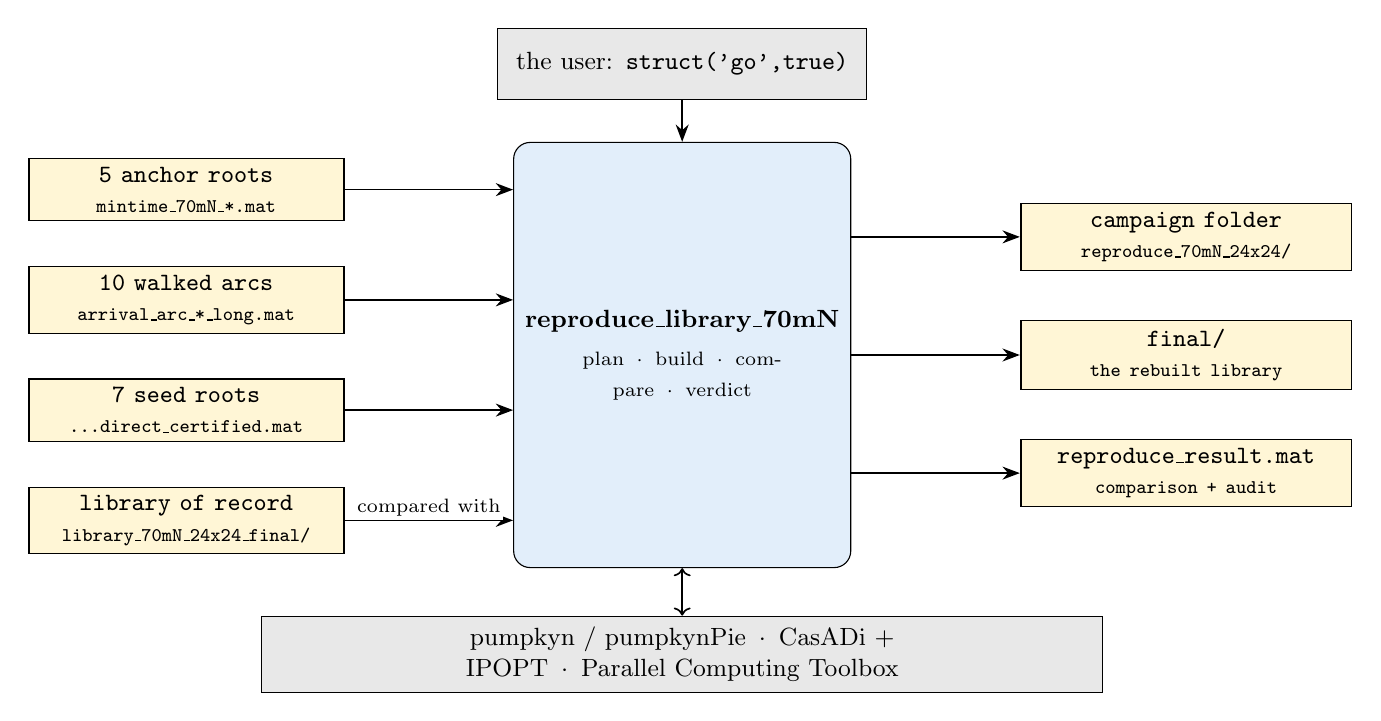
\begin{tikzpicture}
  \node[proc, text width=40mm, minimum height=54mm] (P) at (0,0) {\textbf{reproduce\_library\_70mN}\\[3pt]\scriptsize plan \,$\cdot$\, build \,$\cdot$\, compare \,$\cdot$\, verdict};
  \node[store, text width=38mm] (anch) at (-6.3, 2.1)  {5 anchor roots\\\scriptsize mintime\_70mN\_*.mat};
  \node[store, text width=38mm] (arcs) at (-6.3, 0.7)  {10 walked arcs\\\scriptsize arrival\_arc\_*\_long.mat};
  \node[store, text width=38mm] (seed) at (-6.3,-0.7)  {7 seed roots\\\scriptsize \dots direct\_certified.mat};
  \node[store, text width=38mm] (rec)  at (-6.3,-2.1)  {library of record\\\scriptsize library\_70mN\_24x24\_final/};
  \node[ext,  text width=44mm]  (user) at (0, 3.7) {the user: \code{struct('go',true)}};
  \node[ext,  text width=104mm] (phys) at (0,-3.8) {pumpkyn / pumpkynPie \,$\cdot$\, CasADi + IPOPT \,$\cdot$\, Parallel Computing Toolbox};
  \node[store, text width=40mm] (camp) at (6.4, 1.5)  {campaign folder\\\scriptsize reproduce\_70mN\_24x24/};
  \node[store, text width=40mm] (fin)  at (6.4, 0.0)  {final/\\\scriptsize the rebuilt library};
  \node[store, text width=40mm] (res)  at (6.4,-1.5)  {reproduce\_result.mat\\\scriptsize comparison + audit};
  \draw[flow] (anch.east) -- (anch.east -| P.west);
  \draw[flow] (arcs.east) -- (arcs.east -| P.west);
  \draw[flow] (seed.east) -- (seed.east -| P.west);
  \draw[flow] (rec.east)  -- node[lbl, above]{compared with} (rec.east -| P.west);
  \draw[flow] (user) -- (P);
  \draw[flow, <->] (phys) -- (P);
  \draw[flow] (camp.west -| P.east) -- (camp.west);
  \draw[flow] (fin.west -| P.east)  -- (fin.west);
  \draw[flow] (res.west -| P.east)  -- (res.west);
\end{tikzpicture}
\end{adjustbox}
\caption{System context. The script reads four kinds of file and writes one folder.}
\label{fig:context}
\end{figure}

\paragraph{The inputs, in plain terms.}
\begin{description}[leftmargin=2.2cm, style=nextline, itemsep=2pt]
\item[Anchors] Five certified transfers, all at departure phase 0, one per
  \emph{family} of solutions. A family is one connected branch of the set
  of minimum-time transfers; several families can offer a transfer at the
  same phase pair, and the library keeps the fastest.
  \begin{center}\small
  \begin{tabular}{@{}llll@{}}
  \toprule name & arrival phase & label & how it was found\\\midrule
  \code{anchor} & 0.0754 & fast & the first certified root (2026-09-09)\\
  \code{cell11} & 0.9087 & A2 & the 26-day family\\
  \code{fast2} & 0.8671 & fast2 & found 2026-09-13, faster near 0.87\\
  \code{direct18} & 0.7837 & direct18 & a direct collocation solve at that phase\\
  \code{direct11} & 0.4921 & direct11 & a direct collocation solve at that phase\\
  \bottomrule
  \end{tabular}
  \end{center}
\item[Arcs] From each anchor, the arrival phase was varied continuously in
  both directions (pseudo-arclength continuation), tracing that family.
  An arc stores the whole path, so a sheet at \emph{any} arrival resolution
  can be read off it without walking again. Ten arcs, 2--6 hours each; they
  are most of what a rebuild would otherwise cost.
\item[Seed roots] Seven certified transfers found by direct solves at
  single grid phases, four of them at arrival phases no arc reaches.
\item[Record] The library the rebuild is judged against.
\end{description}

% =========================================================================
\section{Inside the script: six sections}

The function reads top to bottom as six numbered sections
(Figure~\ref{fig:script}). Sections 0--3 only \emph{describe} the build;
in plan mode the function returns after printing them. Section 4 is one
call. Sections 5 and 6 judge the result.

\begin{figure}[h]
\centering
\begin{adjustbox}{max width=\textwidth}
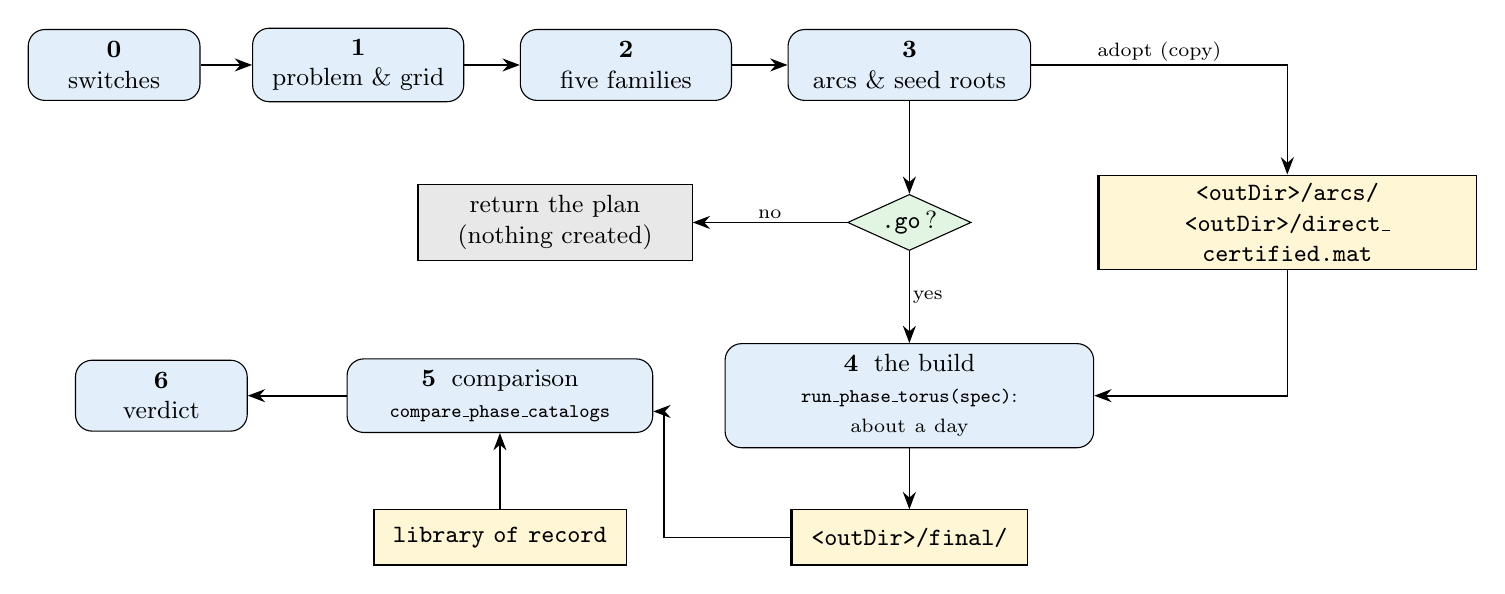
\begin{tikzpicture}
  \node[proc, text width=19mm] (s0) at (0,0)    {\textbf{0}\\switches};
  \node[proc, text width=24mm] (s1) at (3.1,0)  {\textbf{1}\\problem \& grid};
  \node[proc, text width=24mm] (s2) at (6.5,0)  {\textbf{2}\\five families};
  \node[proc, text width=28mm] (s3) at (10.1,0) {\textbf{3}\\arcs \& seed roots};
  \node[gate] (g) at (10.1,-2.0) {\code{.go}\,?};
  \node[ext, text width=32mm] (plan) at (5.6,-2.0) {return the plan\\(nothing created)};
  \node[store, text width=46mm] (adopt) at (14.9,-2.0) {<outDir>/arcs/\\<outDir>/direct\_certified.mat};
  \node[proc, text width=44mm] (s4) at (10.1,-4.2) {\textbf{4}\; the build\\\scriptsize \code{run\_phase\_torus(spec)}: about a day};
  \node[proc, text width=36mm] (s5) at (4.9,-4.2)  {\textbf{5}\; comparison\\\scriptsize \code{compare\_phase\_catalogs}};
  \node[proc, text width=19mm] (s6) at (0.6,-4.2)  {\textbf{6}\\verdict};
  \node[store, text width=28mm] (final)  at (10.1,-6.0) {<outDir>/final/};
  \node[store, text width=30mm] (record) at (4.9,-6.0)  {library of record};
  \draw[flow] (s0) -- (s1); \draw[flow] (s1) -- (s2); \draw[flow] (s2) -- (s3);
  \draw[flow] (s3) -- (g);
  \draw[flow] (g) -- node[lbl, above]{no} (plan);
  \draw[flow] (g) -- node[lbl, right]{yes} (s4);
  \draw[flow] (s3.east) -| node[lbl, pos=0.25, above]{adopt (copy)} (adopt.north);
  \draw[flow] (adopt.south) |- (s4.east);
  \draw[flow] (s4) -- (final);
  \draw[flow] (final.west) -- ++(-1.6,0) |- ([yshift=-2mm]s5.east);
  \draw[flow] (record) -- (s5);
  \draw[flow] (s5) -- (s6);
\end{tikzpicture}
\end{adjustbox}
\caption{The script. \code{spec} is a plain struct handed to the driver; ``adopt'' is a file copy that never overwrites.}
\label{fig:script}
\end{figure}

\begin{description}[leftmargin=1.1cm, style=nextline, itemsep=3pt]
\item[0 -- Switches] The options of the table above.
\item[1 -- Problem and grid] The engine (70\,mN, $I_{sp}$ 900\,s, 150\,kg),
  the DRO of period 1.0 (nondimensional; 4.43 days), the 7-petal southern
  tulip, and the two phase lists: $s_D=k/n_D$ and $s_A$ a lattice through
  the first anchor's phase, 0.0754, \emph{sorted}.
\item[2 -- The five families] The anchor table; each file must exist.
  All five are given, so the driver's discovery step is switched off: it has
  nothing to find, and the run becomes the deterministic part of the build.
\item[3 -- Arcs and seed roots] \code{adopt\_walked\_arcs} copies each arc
  to the name the driver looks for,
  \begin{center}
  \file{results/arrival\_arc\_<name>\_<dn|up>\_long.mat}\\
  $\downarrow$\\
  \file{<outDir>/arcs/arrival\_arc\_70mN\_<name>\_<dn|up>\_long.mat}.
  \end{center} It never overwrites: an identical copy is left alone, a
  different file under that name is an error, a missing source is an error by
  name. The seed-root registry is copied once, because the driver appends to
  it.
\item[4 -- The build] \code{run\_phase\_torus(spec)}; \S\ref{sec:round}.
\item[5 -- Comparison] \S\ref{sec:compare}.
\item[6 -- Verdict] Campaign status, the final catalog's audit, and
  \emph{same library as the record: PASS/FAIL}.
\end{description}

% =========================================================================
\section{One round of the build}\label{sec:round}

\code{run\_phase\_torus} runs \emph{rounds} until a round finds nothing new.
With every family supplied, one round is enough. Figure~\ref{fig:round}
follows the data through it. Every stage writes its product to the round
folder before the next stage starts, so a stopped run resumes at the stage
it was in.

\begin{figure}[h]
\centering
\begin{adjustbox}{max width=\textwidth}
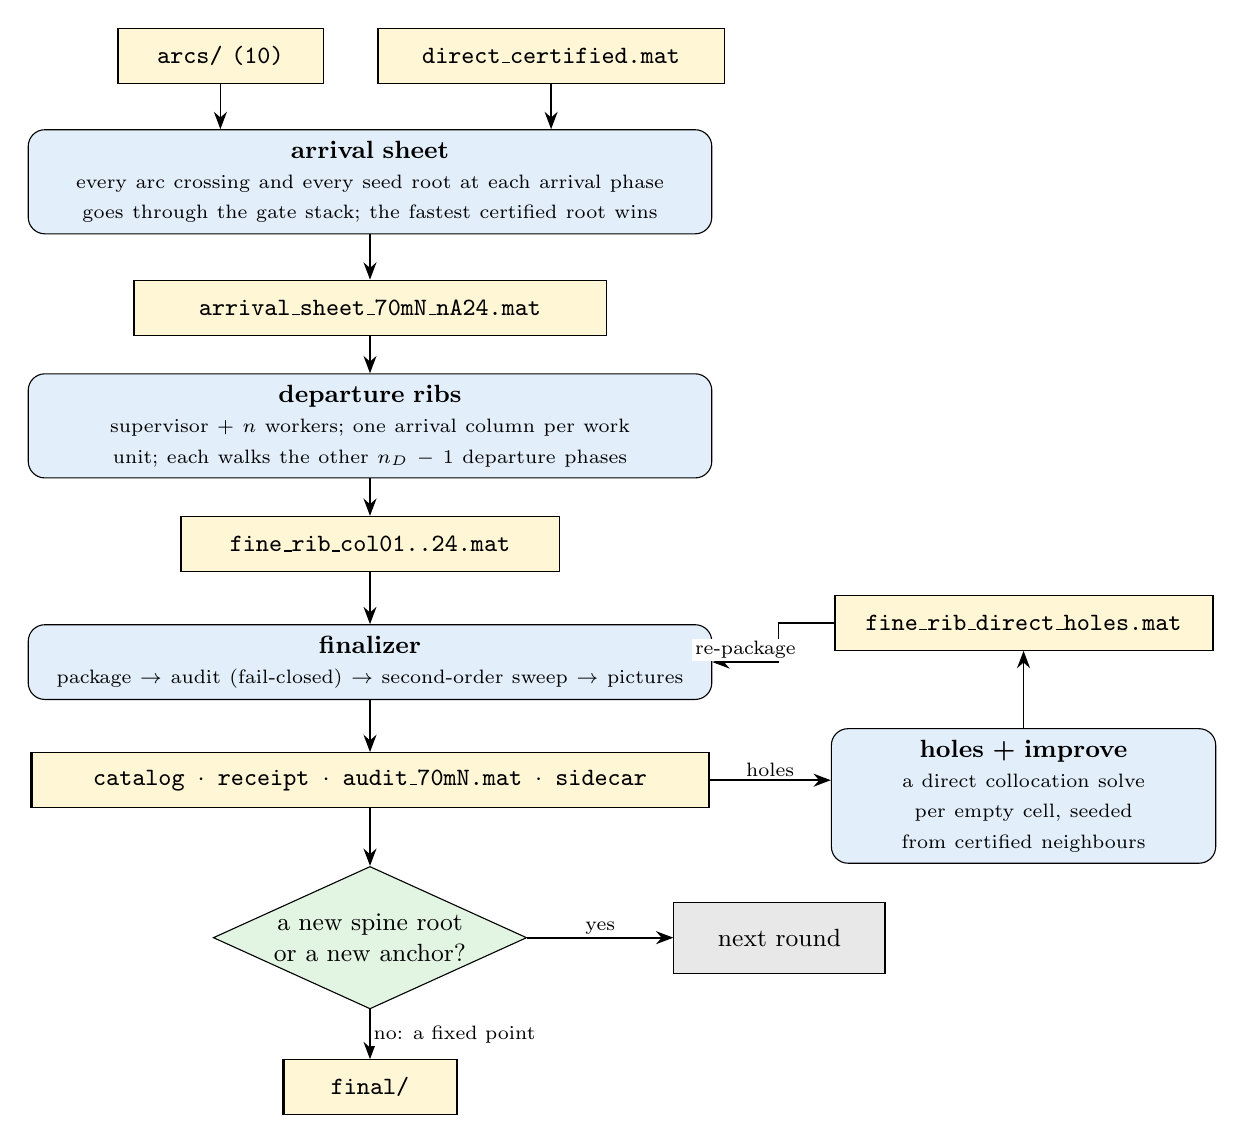
\begin{tikzpicture}
  \node[store, text width=24mm] (arcs) at (-1.9, 0) {arcs/ (10)};
  \node[store, text width=42mm] (reg)  at ( 2.3, 0) {direct\_certified.mat};
  \node[proc, text width=84mm] (sheet) at (0,-1.6) {\textbf{arrival sheet}\\\scriptsize every arc crossing and every seed root at each arrival phase goes through the gate stack; the fastest certified root wins};
  \node[store, text width=58mm] (S) at (0,-3.2) {arrival\_sheet\_70mN\_nA24.mat};
  \node[proc, text width=84mm] (ribs) at (0,-4.7) {\textbf{departure ribs}\\\scriptsize supervisor + $n$ workers; one arrival column per work unit; each walks the other $n_D-1$ departure phases};
  \node[store, text width=46mm] (R) at (0,-6.2) {fine\_rib\_col01..24.mat};
  \node[proc, text width=84mm] (fin) at (0,-7.7) {\textbf{finalizer}\\\scriptsize package $\to$ audit (fail-closed) $\to$ second-order sweep $\to$ pictures};
  \node[store, text width=84mm] (cat) at (0,-9.2) {catalog \,$\cdot$\, receipt \,$\cdot$\, audit\_70mN.mat \,$\cdot$\, sidecar};
  \node[store, text width=46mm] (H) at (8.3,-7.2) {fine\_rib\_direct\_holes.mat};
  \node[proc, text width=46mm] (fill) at (8.3,-9.4) {\textbf{holes + improve}\\\scriptsize a direct collocation solve per empty cell, seeded from certified neighbours};
  \node[gate] (fp) at (0,-11.2) {a new spine root\\or a new anchor?};
  \node[ext, text width=24mm] (again) at (5.2,-11.2) {next round};
  \node[store, text width=20mm] (final) at (0,-13.1) {final/};
  \draw[flow] (arcs) -- (arcs |- sheet.north);
  \draw[flow] (reg) -- (reg |- sheet.north);
  \draw[flow] (sheet) -- (S); \draw[flow] (S) -- (ribs); \draw[flow] (ribs) -- (R);
  \draw[flow] (R) -- (fin); \draw[flow] (fin) -- (cat);
  \draw[flow] (cat.east) -- node[lbl, above]{holes} (cat.east -| fill.west);
  \draw[flow] (fill) -- (H);
  \draw[flow] (H.west) -- ++(-0.7,0) |- node[lbl, pos=0.75, above]{re-package} (fin.east);
  \draw[flow] (cat) -- (fp);
  \draw[flow] (fp) -- node[lbl, above]{yes} (again);
  \draw[flow] (fp) -- node[lbl, right]{no: a fixed point} (final);
\end{tikzpicture}
\end{adjustbox}
\caption{One round. After the filler, the finalizer runs again so the catalog takes in the direct cells; then the driver decides whether another round is needed.}
\label{fig:round}
\end{figure}

\begin{description}[leftmargin=1.1cm, style=nextline, itemsep=3pt]
\item[Arrival sheet (\code{build\_arrival\_sheet})] The row of the library
  at departure phase 0, the \emph{spine}. Each arc is re-scanned where it
  crosses each requested arrival phase; every crossing, and every seed root,
  goes through the gate stack (\S\ref{sec:gates}). Per column the fastest
  certified root is the spine; all candidates are kept.
\item[Ribs (\code{run\_costate\_library}, \code{rib\_from\_crossing})] From
  each spine root the departure phase is walked, one grid step at a time,
  around the DRO. A shell supervisor keeps $n$ MATLAB workers alive; each
  takes the next free column from a work queue, so a slow column delays only
  itself. Every rib point is certified before it is kept.
\item[Finalizer] The supervisor launches it once, when every column is
  published: package the sheet and ribs into a catalog; \emph{audit} the
  catalog as a recipient would; run the \emph{second-order sweep}
  (conjugate-point scan and margins) and write it into the catalog.
\item[Holes and improve (\code{fill\_holes\_direct})] For each empty cell,
  and each cell much slower than its column neighbour, a direct collocation
  solve is warm-started from certified neighbours, its multipliers are
  harvested into a shooting seed, and the result is certified at the exact
  grid phases.
\item[Fixed point] If the round registered no new spine root and added no
  anchor, the campaign is \code{done} and \file{final/} is published.
\end{description}

% =========================================================================
\section{Processes and files}

Several MATLAB processes exist during a build. They never share memory:
\textbf{a file on disk is the only interface between them}, which is why a
killed run loses at most the item in progress (Figure~\ref{fig:procs}).

\begin{figure}[h]
\centering
\begin{adjustbox}{max width=\textwidth}
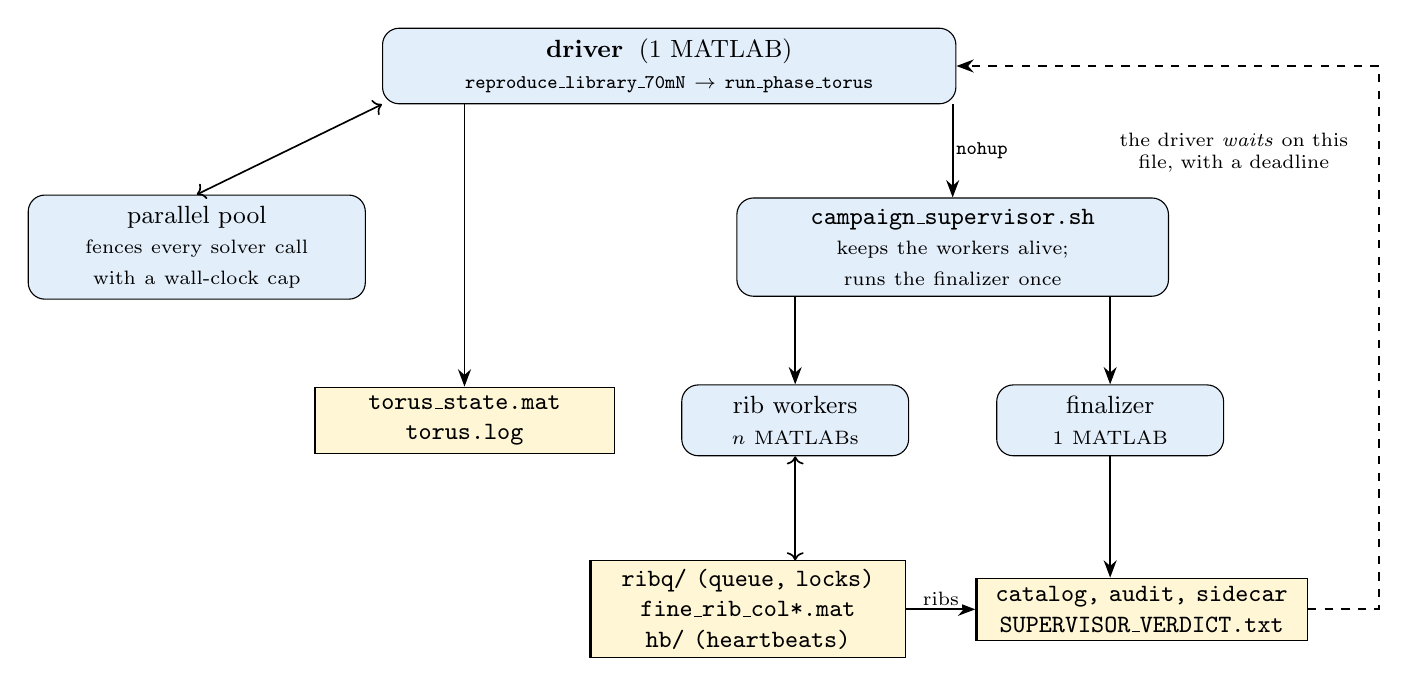
\begin{tikzpicture}
  \node[proc, text width=70mm] (drv) at (0,0) {\textbf{driver} \;(1 MATLAB)\\\scriptsize \code{reproduce\_library\_70mN} $\to$ \code{run\_phase\_torus}};
  \node[proc, text width=40mm] (pool) at (-6.0,-2.3) {parallel pool\\\scriptsize fences every solver call with a wall-clock cap};
  \node[proc, text width=52mm] (sup)  at ( 3.6,-2.3) {\code{campaign\_supervisor.sh}\\\scriptsize keeps the workers alive; runs the finalizer once};
  \node[proc, text width=26mm] (wk) at (1.6,-4.5) {rib workers\\\scriptsize $n$ MATLABs};
  \node[proc, text width=26mm] (fz) at (5.6,-4.5) {finalizer\\\scriptsize 1 MATLAB};
  \node[store, text width=36mm] (st) at (-2.6,-4.5) {torus\_state.mat\\torus.log};
  \node[store, text width=38mm] (q) at (1.0,-6.9) {ribq/ (queue, locks)\\fine\_rib\_col*.mat\\hb/ (heartbeats)};
  \node[store, text width=40mm] (v) at (6.0,-6.9) {catalog, audit, sidecar\\SUPERVISOR\_VERDICT.txt};
  \draw[flow, <->] (drv.south west) -- (pool.north);
  \draw[flow] (drv.south -| st.north) -- (st.north);
  \draw[flow] (drv.south -| sup.north) -- node[lbl, right]{\code{nohup}} (sup.north);
  \draw[flow] (sup.south -| wk.north) -- (wk.north);
  \draw[flow] (sup.south -| fz.north) -- (fz.north);
  \draw[flow, <->] (wk.south) -- (wk.south |- q.north);
  \draw[flow] (fz.south) -- (fz.south |- v.north);
  \draw[flow] (q.east) -- node[lbl, above]{ribs} (v.west);
  \draw[flow, dashed] (v.east) -- ++(0.9,0) |- (drv.east);
  \node[lbl, anchor=east, text width=34mm] at ([xshift=8mm, yshift=58mm]v.east) {the driver \emph{waits} on this file, with a deadline};
\end{tikzpicture}
\end{adjustbox}
\caption{Processes (rounded) and the files between them. The dashed line is a \emph{wait}: the driver polls for the verdict file, with a deadline.}
\label{fig:procs}
\end{figure}

\subsection{The campaign folder}

\begin{center}\small
\begin{tabular}{@{}L{0.44\textwidth}L{0.50\textwidth}@{}}
\toprule
path under \code{<outDir>/} & what it holds \\
\midrule
\file{torus.log} & one line per stage; silent for hours in between \\
\file{torus\_state.mat} & the driver's state: manifest, anchors, rounds, status \\
\file{arcs/} & the arrival arcs (adopted or walked), with \file{.done/.fail/.pid} markers for walked ones \\
\file{direct\_certified.mat} & the registry of certified roots found off the arcs \\
\file{anchors/}, \file{jobs/} & anchors promoted during the run; arc job scripts \\
\file{round\_NN/arrival\_sheet\_*.mat} & the spine with every candidate \\
\file{round\_NN/fine\_rib\_colXX.mat} & one rib file per arrival column \\
\file{round\_NN/ribq/}, \file{hb/}, \file{worker\_*.log} & the work queue, heartbeats, worker logs \\
\file{round\_NN/costate\_catalog\_dro\_tulip\_70mN.mat} & the round's catalog \\
\file{round\_NN/audit\_70mN.mat} & the fail-closed audit of that catalog \\
\file{round\_NN/second\_order\_progress\_v3.mat} & the sweep's sidecar \\
\file{round\_NN/fine\_rib\_direct\_holes.mat}, \file{fill\_holes\_direct.log} & the direct-solved cells \\
\file{final/} & the last round's products: the library \\
\file{reproduce\_result.mat} & the script's output struct: comparison and audit \\
\bottomrule
\end{tabular}
\end{center}

\subsection{The catalog}

One struct with one \emph{sheet}. The fields a reader needs:

\begin{center}\small
\begin{tabular}{@{}L{0.30\textwidth}L{0.17\textwidth}L{0.45\textwidth}@{}}
\toprule
field & size & meaning \\
\midrule
\code{sD\_frac}, \code{sA\_frac} & $1\times n_D$, $1\times n_A$ & the phase lists (the rebuilt library's are \emph{sorted}) \\
\code{has\_solution} & $n_D\times n_A$ & which cells hold an entry \\
\code{tf\_nd} & $n_D\times n_A$ & flight time, nondimensional ($\times\,4.433$ = days) \\
\code{entry\_index}, \code{z8} & $n_D\times n_A$, $8\times N$ & \code{z8(:,entry\_index(i,j))} is the cell's solution \\
\code{conj\_*}, \code{gate\_*}, \code{h6\_margin}, \code{lift\_margin} & $n_D\times n_A$ & second-order and hypothesis measurements \\
\code{family\_index} & $n_D\times n_A$ & provenance: which arc found the entry (nothing reads it) \\
\code{entry\_notes} & $1\times N$ cell & how each entry was found \\
\bottomrule
\end{tabular}
\end{center}

\noindent \textbf{Address cells by phase, not by index.} The hand-built
record listed its arrival phases from the anchor's (0.0754, \dots, 0.9921,
0.0337); the driver sorts them (0.0337 first). Same 24 phases, columns
shifted by one.

% =========================================================================
\section{Certification}\label{sec:gates}

Nothing enters the library without passing \code{certify\_root}, one gate
stack for every route (arc crossing, seed root, rib point, direct solve):

\begin{enumerate}[itemsep=1pt]
\item polish the boundary-value problem (multiple shooting, residual $3\times10^{-11}$);
\item fly the eight numbers alone and require arrival in position \emph{and} velocity;
\item pointwise Pontryagin checks on that flight: $H=0$, transversality, the adjoint equations, the minimum-principle gap;
\item a foreign solver (pumpkyn's \code{tfMin}) must return the same root, and its own flight must arrive;
\item the conjugate-point test passes;
\item the minimum-time hypotheses: $|\lambda_v|>0$ and the throttle switching function $Q_{mt}>0$, as lower-bound \emph{estimates} over the whole arc above a floor of $10^{-5}$; no abnormal lift of the trajectory; condition H6;
\item the dense conjugate scan is clear.
\end{enumerate}

The \textbf{audit} (\code{audit\_phase\_catalog}) then repeats the
recipient's view of the shipped file: rebuild each entry's endpoints from
the catalog's own keys, fly it, re-polish it, recompute the gates. It
\emph{fails closed}: a call that times out, a polished root that moved, a
value that is not a finite scalar, is a BAD row, never a skipped one.
What the certificate does and does not prove is the subject of
\file{doc/mintime\_second\_order\_audit.tex}: it is a numerical assessment
of a \emph{fixed-phase} local-optimality theorem's hypotheses, not a proof,
and says nothing about sliding an endpoint along its orbit.

% =========================================================================
\section{The comparison and the verdict}\label{sec:compare}

\code{compare\_phase\_catalogs(new, reference)} matches cells \emph{by
phase} and reports:

\begin{center}\small
\begin{tabular}{@{}lL{0.72\textwidth}@{}}
\toprule
line & meaning \\
\midrule
grids & if one grid holds all of the other's phases (a $48\times48$ rebuild against the $24\times24$ record) the comparison is made on the shared cells; the rest are counted, not judged \\
coverage & cells one catalog has and the other lacks \\
$t_f$ & flight time within $10^{-6}$ day; otherwise \emph{which catalog is faster} \\
costates & the seven initial costates within $10^{-6}$ relative ($t_f$ is judged on its own line) \\
finite & a NaN is a difference, never a match \\
families & family labels as a \emph{partition}; index numbers do not matter \\
\bottomrule
\end{tabular}
\end{center}

\noindent Two verdicts come out. \code{ok}: the same library. \code{noWorse}:
every reference cell is covered, nothing is non-finite, and no cell is
slower. The script prints \textbf{REPRODUCED: PASS} only if \code{ok} holds
\emph{and} the final catalog's own audit covers every entry with no BAD row.

\paragraph{The first result.} 565 cells the same root; 11 cells a different
root, the rebuild faster in all 11 by 1.95--3.93 days; 82 cells the same
root under another family label. Strict verdict FAIL, \code{noWorse} true.
For a minimum-time library that is a better library, and it was adopted as
the record. The label differences are not differences in the solutions: rib
labels are attached by flight time and are not reproducible between builds.

% =========================================================================
\section{How long it takes}

Measured on the first rebuild (4 rib workers):

\begin{center}\small
\begin{tabular}{@{}lrl@{}}
\toprule
stage & time & scales with \\
\midrule
arrival sheet ($\approx$300 candidates) & 1\,h 34 & $n_A$ \\
ribs (24 columns $\times$ 23 points) & $\approx$9\,h & $n_A(n_D-1)$ / workers \quad (235 worker-seconds per point)\\
package, audit, sweep (519 entries) & $\approx$4\,h & $n_Dn_A$ \quad (28\,s per entry)\\
holes and improve (58 cells) & 7\,h & $\approx10\%$ of cells, 7.2\,min each \\
re-package, audit again, sweep & 2\,h 31 & $n_Dn_A$ \quad (15.7\,s per entry)\\
\midrule
\textbf{total} & \textbf{24\,h 12} & \\
\bottomrule
\end{tabular}
\end{center}

\noindent The script prints an estimate from these rates before it builds:
24.5\,h for $24\times24$ (measured 24.2), 96\,h for $48\times48$ or
$24\times96$. The driver's wait for a round scales the same way (three
times the estimate, never under 48\,h); it used to be a flat 48\,h, which a
$48\times48$ round would have outlived. The first estimate ever quoted for
this script was ``6--10 hours''. It was a guess.

% =========================================================================
\section{Running it unattended}

\begin{enumerate}[itemsep=2pt]
\item \textbf{Rehearse} after any change under the driver: the $3\times3$
  acceptance case reaches a fixed point in two rounds and about 90 minutes,
  and its catalog should equal \file{results/torus3d\_p0/final} cell for
  cell. Fast tests do not prove a live round.
\item \textbf{Launch detached}, never in the interactive session:
  \file{indirect/batch/reproduce\_library\_job.m} builds the path, calls the
  script inside a \code{try/catch}, saves the result and writes a one-line
  verdict file whether it succeeded or threw.
\item \textbf{Watch} \file{torus.log} (one line per stage), the job's output
  (per-candidate and per-audit-row lines), and the verdict file or the death
  of the process. Hours of silence in \file{torus.log} are normal.
\item \textbf{Resume} by calling it again with the same options.
\end{enumerate}

% =========================================================================
\section{Failure handling, and known limitations}

\paragraph{What is handled.} A failed arc writes a verdict file and stops
the campaign at once; a MATLAB that dies before its own error handling is
caught by a shell wrapper that writes the verdict for it. A rib column that
fails repeatedly is retired and reported, not retried forever. A catalog is
accepted only if packaging, audit and sweep all passed. A budget-limited
campaign resumes when the budget is raised.

\paragraph{What is not} (external review, 2026-09-18; these bite an
\emph{interrupted} run, not a fresh one). Final publication is not
transactional, and the campaign's status is saved before \file{final/}
exists. The fixed-point decision uses the current call's counters, so a
resumed round can declare \code{done} on a sheet that predates a registered
root. A recorded process id is ``alive'', not ``ours''. Arc adoption checks
bytes, not the arc's identity. The audit is tied to the final catalog by
location and entry count, not by a content hash. After an interruption,
prefer a fresh \code{outDir}.

\paragraph{Seven traps this work fell into.} Two files named
\file{run\_costate\_library.m}; the phase ordering above; the audit file's
name follows the packaging chain's tag, not the driver's; MATLAB struct
arrays need one field set on every return path; \code{NaN > tol} is false,
so an unvalidated comparison passes NaN; a bulk substring rename also renamed
a function definition; an idle parallel pool times out and the certifier
then refuses to run.

% =========================================================================
\section{Modules and their tests}

\begin{center}\small
\begin{tabular}{@{}L{0.34\textwidth}L{0.30\textwidth}L{0.30\textwidth}@{}}
\toprule
file (\file{indirect/} unless noted) & role & test \\
\midrule
\file{reproduce\_library\_70mN.m} & this script & \file{test\_reproduce\_library} \\
\file{compare\_phase\_catalogs.m} & the comparison & same \\
\file{adopt\_walked\_arcs.m} & arc adoption & same \\
\file{run\_phase\_torus.m} & the round-loop driver & \file{test\_run\_phase\_torus\_p0} \\
\file{run\_costate\_library.m} & one round's front door & \file{test\_run\_costate\_library\_seams} \\
\file{build\_arrival\_sheet.m}, \file{sheet\_from\_arcs.m} & the spine & \file{test\_sheet\_from\_arcs}, \file{test\_crossings\_from\_arc} \\
\file{rib\_from\_crossing.m}, \file{build\_ribs.m} & the ribs & \file{test\_rib\_from\_crossing} \\
\file{fill\_holes\_direct.m}, \file{direct\_cell\_solve.m} & the filler & \file{test\_fill\_holes\_physics} \\
\file{certify\_root.m} & the gate stack & \file{test\_certify\_enforcement}, \file{test\_certify\_schema} \\
\file{audit\_phase\_catalog.m} & the fail-closed audit & \file{test\_audit\_fail\_closed} \\
\file{family\_map.m} & families; root identity by costates & \file{test\_family\_map}, \file{test\_family\_costate\_identity} \\
\file{phase\_transversality\_check.m} & costates against a finite-difference test & \file{test\_phase\_transversality\_check} \\
\file{build\_70mN\_library.m} & \emph{only} the packager now (stages 5--8) & --- \\
\bottomrule
\end{tabular}
\end{center}

\noindent Local helper functions are reached by tests through one seam:
\code{H = some\_file('localfunctions')} returns handles to that file's
local functions, so a test calls the real helper and not a copy of it.

% =========================================================================
\section{Extending it}\label{sec:extend}

\paragraph{Another resolution.} \code{struct('go',true,'nD',48,'nA',48)}.
The arcs are re-scanned at any arrival resolution and the comparison is made
on the shared cells. Expect about four days. Note that the two axes are not
alike: along departure phase the library is already smooth at 24 phases,
while along arrival phase the flight time is under-resolved (a 7-petal tulip
puts structure at a seventh of a period). If the purpose is interpolation,
refine $n_A$, not $n_D$.

\paragraph{Another orbit pair or engine.} Not yet one call. The pipeline
under the driver is wired to three numbers (\code{tauDRO}, \code{NpTulip},
\code{pmTulip}) and every identity check copies that list. The route is an
orbit-pair object (two phase-to-state closures, two periods, two names)
carried as the problem identity; a first certified root of the new problem
(\code{anchor\_by\_direct\_solve}); and the driver walking its own arcs with
discovery on. The record of that analysis is
\file{reviews/library\_pipeline\_and\_optimality\_adjudicated\_2026-09-17.md}.

\section*{Where to read more}
\begin{itemize}[itemsep=1pt]
\item \file{process/REPRODUCE\_LIBRARY\_GUIDE.md}: the operator's guide.
\item \file{process/PHASE\_TORUS\_RUNBOOK.md}: the hand-driven process this replaces.
\item \file{FINDINGS.md} sections 78--84: how the script came to be, the reviews, the first rebuild.
\item \file{doc/mintime\_second\_order\_audit.tex}: what the certificate means.
\end{itemize}

\end{document}
